\documentclass[a4paper,10pt]{article}
\usepackage{a4wide}
\usepackage[T1]{fontenc}
\usepackage[utf8]{inputenc}
\usepackage[english]{babel}

\usepackage{xfrac} 				% gives \sfrac
\usepackage{amsmath}
\usepackage{enumerate} 		% allows you to change counters
\usepackage{verbatim}
\usepackage{comment}				% gives comment environment
\usepackage{hyperref}
\usepackage{amssymb}				% gives f.x. \mathbb{R}

% graphics packages
\usepackage{graphicx}
\usepackage{caption} 	
\usepackage{subcaption}
\usepackage{float}

\title{
	Assignment 2 - Basic Learning Algorithms	\\
	Statistical Methods for Machine Learning
  }
\author{
	Guðmundur Páll Kjartansson \\
	Jón Gísli Egilsson
}

% Uncomment to set paragraph indentation to 0 points, and skips a line
% after an ended paragraph.
\setlength{\parindent}{0pt}
\setlength{\parskip}{\baselineskip}

\begin{document}
\maketitle

\section*{II.1 Regression}

\subsection*{II.1.1 Maximum likelihood solution}

The models for variable selections $1$ and $2$ are implemented in the file \verb=regression.py=. We then applied both models to the test set and computed the RMS averaged over $100$ different selections of training and test data (where the training data was always $80\%$ and test data $20\%$ of the data in the file \verb=bodyfat.txt=). Our measured RMS errors for selection $1$ and $2$ respectively were
$$\text{RMS}_1 \approx 4.5$$
and
$$\text{RMS}_2 \approx 5.$$

\subsection*{II.1.2 Maximum a posteriori solution}

We also implemented the MAP estimate in \verb=regression.py=. In figure $1$ we can see the RMS error for the MAP estimate plotted for different values of the precision parameter $\alpha$. The RMS for the maximum likelihood solution was included in the plot for the same dataset for comparison.

Comparing the selections we see that selection $1$ seems to provide better prediction than selection $2$ given the minimizing $\alpha$ value. And if we chose $\alpha$ to be anywhere between $0$ and $0.1$ (not including $0$) we will get better results with the MAP estimate than the ML one. Similarly if we have $0 < \alpha \leq 0.24$ for selection $2$ the MAP provides better prediction than the ML one.

\begin{figure}[H]
	\centering
	\begin{subfigure}{0.45\textwidth}
  		\centering
  		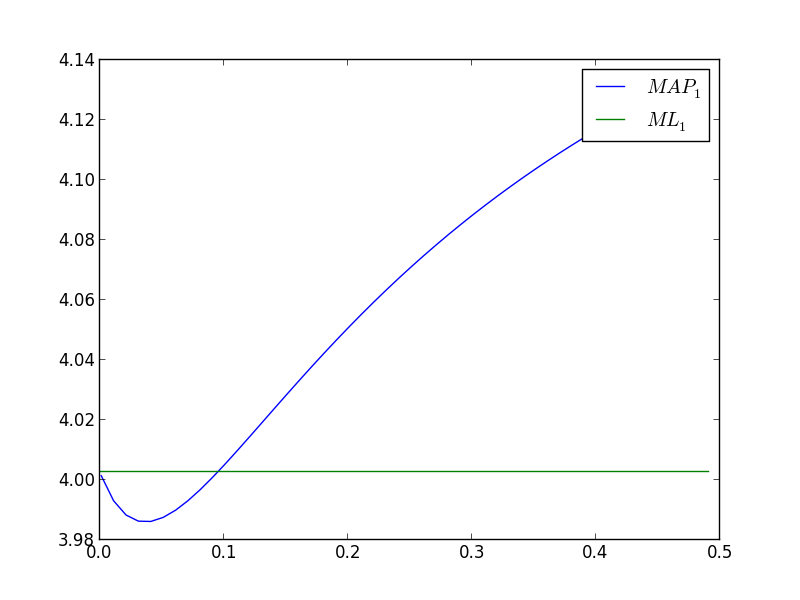
\includegraphics[width=\textwidth]{../images/report/rms_selection1.png}
  		\caption{Selection $1$}
  \end{subfigure}
  \begin{subfigure}{0.45\textwidth}
  		\centering
  		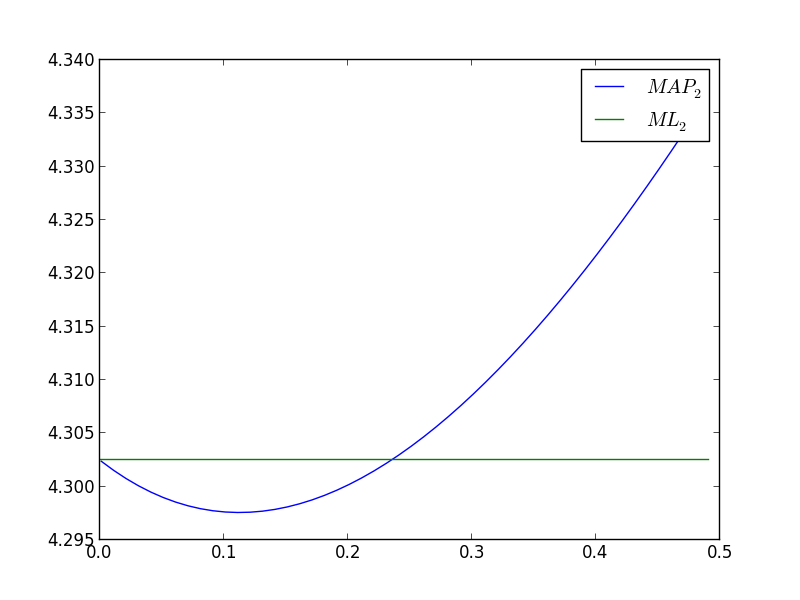
\includegraphics[width=\textwidth]{../images/report/rms_selection2.png}
  		\caption{Selection $2$}
  \end{subfigure}
  	\caption{RMS for MAP and ML}
\end{figure}

\subsection*{II.1.3 Maximum a posteriori solution}

We want to prove that 
$$p(w|t) = \mathcal{N}(w|m_N,S_N)$$
where
\begin{align*}
m_N &= S_N(S_0^{-1}m_0 + \beta \Phi^Tt) \\
S_N^{-1} &= S_0^{-1} + \beta \Phi^T \Phi.
\end{align*}
Now we see that
\begin{align*}
\ln(p(w|t)) &\propto \ln(p(w)p(t|w)) \\
		&= \ln(\mathcal{N}(w|m_0,S_0)) + \ln\left(\prod_{n=1}^N \mathcal{N}(t_n|w^T\phi(x_n),\beta^{-1})\right) \\
		&= -\frac{1}{2}(w-m_0)^T S_0^{-1} (w-m_0) + \sum_{n=1}^N \left( -\frac{1}{2}(t_n-w^T\phi(x_n))^T \beta (t_n-w^T\phi(x_n)) \right).
\end{align*}
Here we consider that $S_0^{-1} = \alpha I$ and $m_0 = 0$ we get by continuing from above that
\begin{align*}
\ln(p(w|t)) &\propto -\frac{1}{2}w^T \alpha I w + -\frac{1}{2}(t-\Phi w)^T \beta (t-\Phi w) \\
		&= -\frac{1}{2}\left( w^T \alpha I w + t^T\beta t - t^T \beta \Phi w - w^T\Phi^T \beta t + w^T \Phi^T \beta \Phi w \right) \\
		&\propto -\frac{1}{2}\left( w^T (\alpha I + \beta \Phi^T \Phi) w - \beta t^T  \Phi w - \beta w^T\Phi^T t \right) \\
		&= -\frac{1}{2}\left( w^T S_N^{-1} w - \beta t^T  \Phi w - \beta w^T\Phi^T t \right) \quad (\ast).
\end{align*}
Now we will note that 
\begin{align*}
\ln(\mathcal{N}(w|m_N,S_N)) &= -\frac{1}{2} (w - S_N(S_0^{-1}m_0 + \beta \Phi^Tt))^T S_N^{-1}(w - S_N(S_0^{-1}m_0 + \beta \Phi^Tt)) \\
		&\propto -\frac{1}{2}\left( w^T S_N^{-1} w - \beta (S_N\Phi^T t)^T S_N^{-1} w - \beta w^T S_N^{-1} S_N \Phi^T t \right) \\
		&= -\frac{1}{2}\left( w^T S_N^{-1} w - \beta t^T \Phi S_N^T S_N^{-1} w - \beta w^T S_N^{-1} S_N \Phi^T t \right)
\end{align*}
We know that $S_N$ is a symmetric matrix so $S_N^T = S_N$ and $S_N^T S_N^{-1} = I$. Then
$$\ln(\mathcal{N}(w|m_N,S_N)) \propto -\frac{1}{2}\left( w^T S_N^{-1} w - \beta t^T \Phi w - \beta w^T \Phi^T t \right)$$
which is the same result as we got in $(\ast)$. Thus we have shown that
$$p(w|t) = \mathcal{N}(w|m_N,S_N).$$


\section*{II.2 Classification}

\subsection*{II.2.1 Linear discriminant analysis}

We implemented the linear discriminant analysis algorithm in \verb=classification.py=. In figure $2$ we can see the three different classes in the training data.
\begin{figure}[H]
	\centering
  		\centering
  		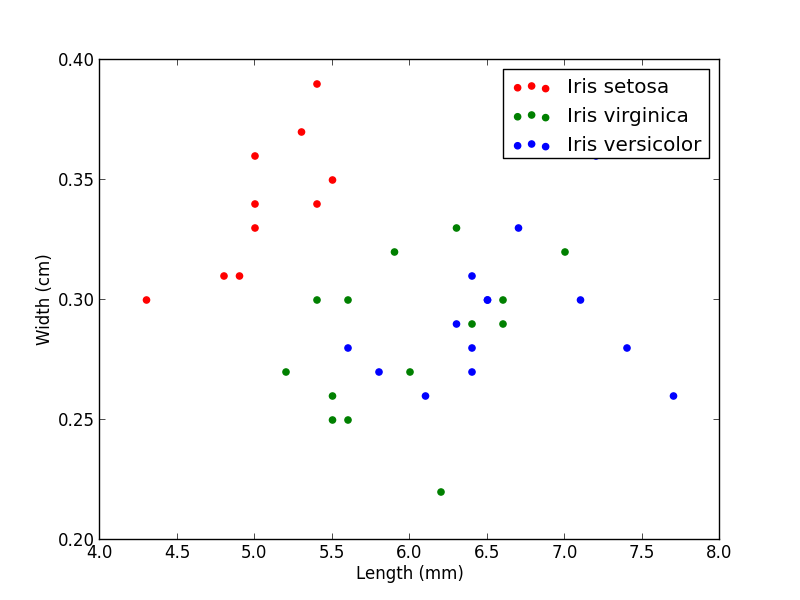
\includegraphics[width=0.6\textwidth]{../images/report/iris_scatter.png}
  		\caption{Scatter plot of Iris data}
\end{figure}
Now to quantify the error of the LDA we compute the probability of misclassification for the training and test data respectively. The errors are
$$\epsilon_{\text{training}} = 0.21$$
and
$$\epsilon_{\text{test}} = 0.18.$$

\subsection*{II.2.5 LDA with rescaled data}

The rescaled data with $M$ can be found in the files \verb=irisTrain.dt.scaled= and \verb=irisTest.dt.scaled=. The training and test errors we get for this transformed data are the same as we got before the transformation or 
$$\epsilon_{\text{training}} = 0.21$$
and
$$\epsilon_{\text{test}} = 0.18.$$
The short answer to \emph{why} we get the same errors is \emph{linearity}. This transformation by $M$ is just rescaling of the $y$-axis.


\begin{comment}
\begin{figure}[H]
	\centering
	\begin{subfigure}{0.45\textwidth}
  		\centering
  		\includegraphics[width=\textwidth]{../week4/images/prob41asurf.png}
  		\caption{$x=(0,-1)$}
  \end{subfigure}
  \begin{subfigure}{0.45\textwidth}
  		\centering
  		\includegraphics[width=\textwidth]{../week4/images/prob41bsurf.png}
  		\caption{$x=(0,0.05)$}
  \end{subfigure}
  	\caption{Surface plots of $m(p)$ at different points}
\end{figure}
\end{comment}


\end{document}




































